% Options for packages loaded elsewhere
\PassOptionsToPackage{unicode}{hyperref}
\PassOptionsToPackage{hyphens}{url}
%
\documentclass[
]{book}
\usepackage{lmodern}
\usepackage{amsmath}
\usepackage{ifxetex,ifluatex}
\ifnum 0\ifxetex 1\fi\ifluatex 1\fi=0 % if pdftex
  \usepackage[T1]{fontenc}
  \usepackage[utf8]{inputenc}
  \usepackage{textcomp} % provide euro and other symbols
  \usepackage{amssymb}
\else % if luatex or xetex
  \usepackage{unicode-math}
  \defaultfontfeatures{Scale=MatchLowercase}
  \defaultfontfeatures[\rmfamily]{Ligatures=TeX,Scale=1}
\fi
% Use upquote if available, for straight quotes in verbatim environments
\IfFileExists{upquote.sty}{\usepackage{upquote}}{}
\IfFileExists{microtype.sty}{% use microtype if available
  \usepackage[]{microtype}
  \UseMicrotypeSet[protrusion]{basicmath} % disable protrusion for tt fonts
}{}
\makeatletter
\@ifundefined{KOMAClassName}{% if non-KOMA class
  \IfFileExists{parskip.sty}{%
    \usepackage{parskip}
  }{% else
    \setlength{\parindent}{0pt}
    \setlength{\parskip}{6pt plus 2pt minus 1pt}}
}{% if KOMA class
  \KOMAoptions{parskip=half}}
\makeatother
\usepackage{xcolor}
\IfFileExists{xurl.sty}{\usepackage{xurl}}{} % add URL line breaks if available
\IfFileExists{bookmark.sty}{\usepackage{bookmark}}{\usepackage{hyperref}}
\hypersetup{
  pdftitle={Statistics with jamovi},
  pdfauthor={Dana Wanzer},
  hidelinks,
  pdfcreator={LaTeX via pandoc}}
\urlstyle{same} % disable monospaced font for URLs
\usepackage{longtable,booktabs}
% Correct order of tables after \paragraph or \subparagraph
\usepackage{etoolbox}
\makeatletter
\patchcmd\longtable{\par}{\if@noskipsec\mbox{}\fi\par}{}{}
\makeatother
% Allow footnotes in longtable head/foot
\IfFileExists{footnotehyper.sty}{\usepackage{footnotehyper}}{\usepackage{footnote}}
\makesavenoteenv{longtable}
\usepackage{graphicx}
\makeatletter
\def\maxwidth{\ifdim\Gin@nat@width>\linewidth\linewidth\else\Gin@nat@width\fi}
\def\maxheight{\ifdim\Gin@nat@height>\textheight\textheight\else\Gin@nat@height\fi}
\makeatother
% Scale images if necessary, so that they will not overflow the page
% margins by default, and it is still possible to overwrite the defaults
% using explicit options in \includegraphics[width, height, ...]{}
\setkeys{Gin}{width=\maxwidth,height=\maxheight,keepaspectratio}
% Set default figure placement to htbp
\makeatletter
\def\fps@figure{htbp}
\makeatother
\setlength{\emergencystretch}{3em} % prevent overfull lines
\providecommand{\tightlist}{%
  \setlength{\itemsep}{0pt}\setlength{\parskip}{0pt}}
\setcounter{secnumdepth}{5}
\usepackage{booktabs}

\newenvironment{danger}
    {
    \hline\\
    }
    { 
    \\\\\hline
    }
    
\newenvironment{warning}
    {
    \hline\\
    }
    { 
    \\\\\hline
    }
    
\newenvironment{info}
    {
    \hline\\
    }
    { 
    \\\\\hline
    }
    
\newenvironment{try}
    {
    \hline\\
    }
    { 
    \\\\\hline
    }
\ifluatex
  \usepackage{selnolig}  % disable illegal ligatures
\fi
\usepackage[]{natbib}
\bibliographystyle{apalike}

\title{Statistics with jamovi}
\author{Dana Wanzer}
\date{Last Update: 2020-10-24}

\begin{document}
\maketitle

{
\setcounter{tocdepth}{1}
\tableofcontents
}
\hypertarget{welcome}{%
\chapter*{Welcome}\label{welcome}}
\addcontentsline{toc}{chapter}{Welcome}

This is the website for PSYC 290 and PSYC 790 at the University of Wisconsin-Stout, taught by Dana Wanzer. These resources are aimed at teaching you how to use jamovi and null hypothesis significance testing (NHST) to answer research questions.

This website is \textbf{free to use} and is licensed under a Creative Commons BY-SA (CC BY-SA) license version 4.0. This means you are free to \textbf{share} (i.e., copy and redistribute the material in any medium or format) and \textbf{adapt} (i.e., remix, transform, and build upon the material for any purpose, even commercially), provided that you \textbf{attribute} these resources by citing me, indicating if changes were made and you \textbf{share alike} (i.e., if you adapt, you must distribute your contributes under the same license as the original).

Portions of this book may have been adapted from ``\href{http://www.learnstatswithjamovi.com}{Learning statistics with jamovi: A tutorial for psychology students and other beginners}'' by Danielle J. Navarro and David R. Foxcroft, version 0.70. Furthermore, the template and style of this book is from \href{https://psyteachr.github.io/book-template/setup.html}{PsyTeachR}.

\hypertarget{introduction}{%
\chapter{Introduction}\label{introduction}}

This chapter will walk you through how this website/book works.

\hypertarget{quiz-questions}{%
\section{Quiz Questions}\label{quiz-questions}}

Throughout this website, there will be questions to help you test your knowledge. When you type in or select the correct answer, the dashed box will change color and become solid.

For example:

\begin{itemize}
\item
  What is 2+2?
\item
  We attend the University of Wisconsin- Stout Madison Green Bay
\item
  True or false: Statistics is awesome. TRUE FALSE
\end{itemize}

\hypertarget{errors-and-mistakes}{%
\section{Errors and mistakes}\label{errors-and-mistakes}}

I am human, therefore I err. If you find an error in the textbook or something you think might be a mistake, please let me know ASAP so I can update this for everyone else. Let me know which section you find the error or mistake in and what the error or mistake is. For example, if there was an error here you could say, ``There was an error in 1.2 that the first sentence should really be `To err is human.'\,''

\hypertarget{independent-t-test}{%
\chapter{Independent t-test}\label{independent-t-test}}

\hypertarget{what-is-the-independent-t-test}{%
\section{What is the independent t-test?}\label{what-is-the-independent-t-test}}

The independent t-test is used to test the difference in our dependent variable between two different groups of observations. Our grouping variable is our independent variable. In other words, we use the independent t-test when we have a research question with a \textbf{continuous dependent variable} and a \textbf{categorical independent variable with two categories in which different participants are in each category}.

The independent t-test is also the independent samples t-test and the Student's t-test. I will use these terms interchangeably.

\hypertarget{data-set-up}{%
\section{Data set-up}\label{data-set-up}}

To conduct the independent t-test, we first need to ensure our data is set-up properly in our dataset. This requires having two columns: one with our continuous dependent variable and one indicating which group the participant is in. Each row is a unique participant or unit of analysis. Here's what example data may look like if we were testing for differences in a test score by students in my fall or spring semesters of this course:

\begin{longtable}[]{@{}llr@{}}
\caption{Example data for the independent t-test}\tabularnewline
\toprule
ID & Semester & TestScore\tabularnewline
\midrule
\endfirsthead
\toprule
ID & Semester & TestScore\tabularnewline
\midrule
\endhead
1 & Fall & 86\tabularnewline
2 & Fall & 80\tabularnewline
3 & Fall & 75\tabularnewline
4 & Fall & 79\tabularnewline
5 & Fall & 82\tabularnewline
6 & Spring & 84\tabularnewline
7 & Spring & 90\tabularnewline
8 & Spring & 72\tabularnewline
9 & Spring & 75\tabularnewline
10 & Spring & 81\tabularnewline
\bottomrule
\end{longtable}

In the example data above, what is your \textbf{independent variable}? ID Semester TestScore

In the example data above, what is your \textbf{dependent variable}? ID Semester TestScore

\hypertarget{the-math-behind-the-independent-t-test}{%
\section{The math behind the independent t-test}\label{the-math-behind-the-independent-t-test}}

The basic math of the independent t-test the mean difference divided by the pooled standard error.

\(t = \frac{\bar{X}_1 - \bar{X}_2}{SE({\bar{X}_1 - \bar{X}_2})}\)

The denominator of the equation is more difficult to calculate and depends on whether the sample size between groups is equal.

\hypertarget{assumptions}{%
\section{Assumptions}\label{assumptions}}

As a parametric test, the independent t-test has the same assumptions as other parametric tests:

\begin{enumerate}
\def\labelenumi{\arabic{enumi}.}
\item
  The dependent variable is \textbf{normally distributed}
\item
  Variances in the two groups are roughly equal (i.e., \textbf{homogeneity of variances})
\item
  The dependent variable is \textbf{interval or ratio} (i.e., continuous)
\item
  Scores are \textbf{independent} between groups
\end{enumerate}

We cannot \underline{test} the third and fourth assumptions; rather, those are based on knowing your data.

However, we can and should test for the first two assumptions. Fortunately, the independent samples t-test in jamovi has two check boxes under ``Assumption Checks'' that lets us test for both assumptions.

\hypertarget{in-jamovi}{%
\section{In jamovi}\label{in-jamovi}}

Let's run an example with data from lsj-data. Open data from your Data Library in ``lsj-data''. Select and open ``Harpo''. This dataset is hypothetical data of 33 students taking Dr.~Harpo's statistics lectures. We have two tutors for the class, Anastasia (\emph{n} = 15) and Bernadette (\emph{n} = 18). Our research question is ``Which tutor results in better student grades?'' We don't have a hypothesis that one does better than the other.

\begin{enumerate}
\def\labelenumi{\arabic{enumi}.}
\item
  To perform an independent t-test in jamovi, go to the Analyses tab, click the T-Tests button, and choose ``Independent Samples T-Test''.
\item
  Move your dependent variable \texttt{grade} to the Dependent Variables box and your independent variable \texttt{tutor} to the Grouping Variable box.
\item
  Under Tests, select \texttt{Student\textquotesingle{}s}
\item
  Under Hypothesis, because we have a two-sided hypothesis select a two-sided hypothesis (Group 1 does not equal Group 2).
\item
  Under Additional Statistics, select \texttt{Mean\ difference}, \texttt{Effect\ size}, and \texttt{Descriptives}.
\item
  Under Assumption Checks, select all three options: \texttt{Homogeneity\ test}, \texttt{Normality\ test}, and \texttt{Q-Q\ plot}.
\end{enumerate}

When you are done, your setup should look like this

\begin{figure}

{\centering 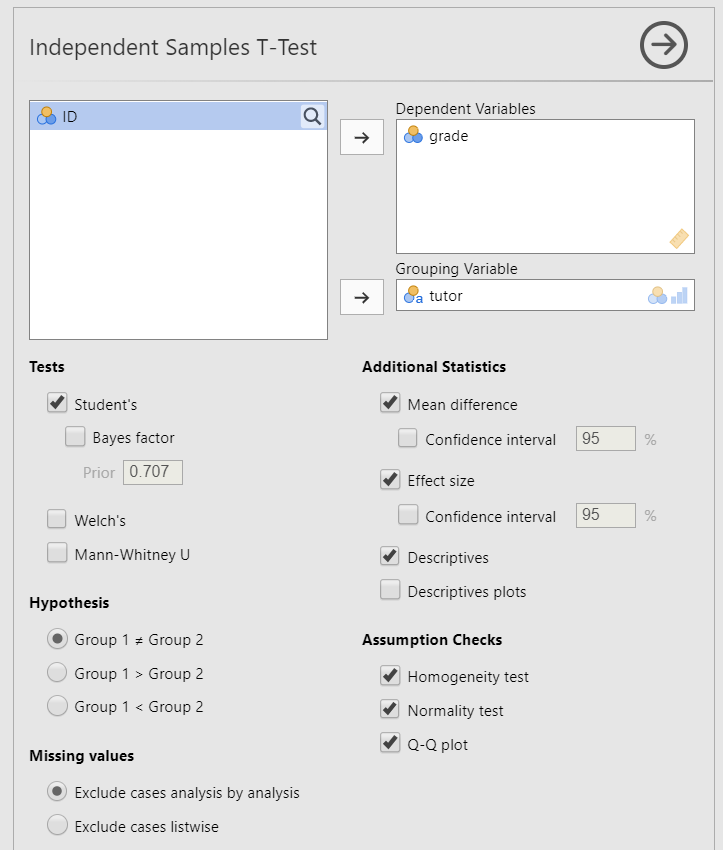
\includegraphics[width=0.8\linewidth]{images/02-independent_t-test/independent_t-test_setup} 

}

\caption{Independent t-test setup in jamovi}\label{fig:unnamed-chunk-1}
\end{figure}

\hypertarget{checking-assumptions-in-jamovi}{%
\subsection{Checking assumptions in jamovi}\label{checking-assumptions-in-jamovi}}

\hypertarget{testing-normality}{%
\subsubsection{Testing normality}\label{testing-normality}}

We test for normality using the Shapiro-Wilk test and the Q-Q plot. The Shapiro-Wilk test was not statistically significant (W = .98, \emph{p} = .827); therefore, this indicates the data is normally distributed. Furthermore, the lines are fairly close to the diagonal line in the Q-Q plot. We can conclude that we satisfy the assumption of normality.

\begin{figure}

{\centering 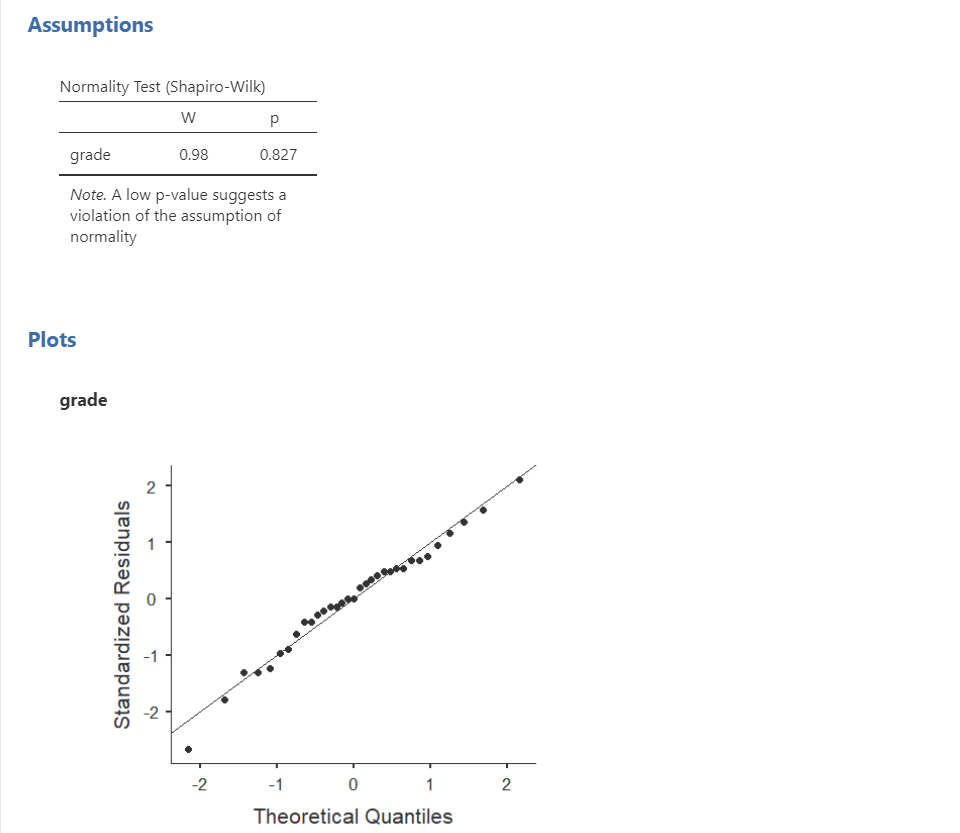
\includegraphics[width=1\linewidth]{images/02-independent_t-test/independent_t-test_normality} 

}

\caption{Testing normality in jamovi}\label{fig:unnamed-chunk-2}
\end{figure}

\hypertarget{testing-homogeneity-of-variance}{%
\subsubsection{Testing homogeneity of variance}\label{testing-homogeneity-of-variance}}

We test for homogeneity of variance using the Levene's test. The Levene's test was not statistically significant (\emph{F} {[}1, 31{]} = 2.49, \emph{p} = .125); therefore, this indicates our data satisfies the assumption of homogeneity of variance. However, I would add a caveat that we have a small sample of data (\emph{n} = 15 for Anastasia and \emph{n} = 18 for Bernadette) and the standard deviations are quite different from one another (SD = 9.00 vs 5.77, respectively). We should have tried to collect more data.

\begin{figure}

{\centering 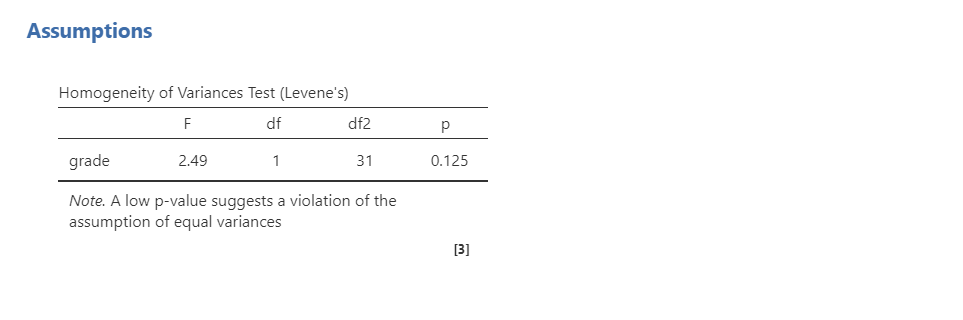
\includegraphics[width=1\linewidth]{images/02-independent_t-test/independent_t-test_homogeneity} 

}

\caption{Testing homogeneity of variance in jamovi}\label{fig:unnamed-chunk-3}
\end{figure}

\hypertarget{interpreting-results}{%
\subsection{Interpreting results}\label{interpreting-results}}

Once we are satisfied we have satisfied the assumptions for the independent t-test, we can interpret our results.

\begin{figure}

{\centering 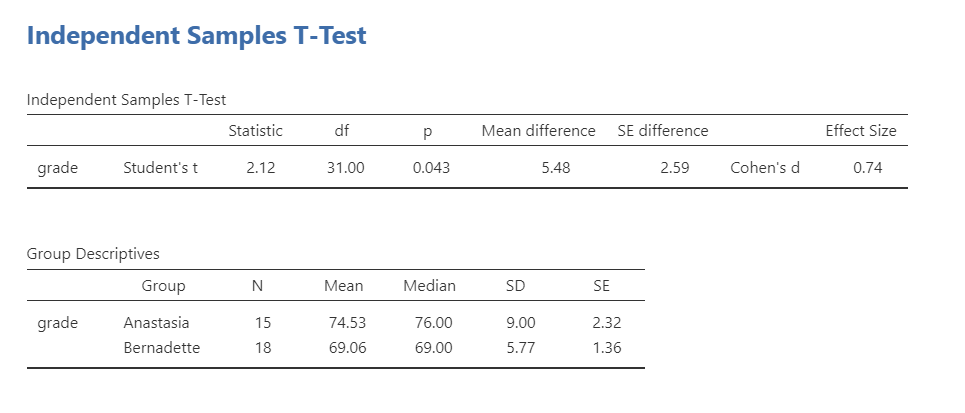
\includegraphics[width=1\linewidth]{images/02-independent_t-test/independent_t-test_ind-results} 

}

\caption{Independent t-test results in jamovi}\label{fig:unnamed-chunk-4}
\end{figure}

Our p-value is less than .05, so our results are statistically significant. We can write up our results in APA something like this:

\begin{quote}
Anastasia's students (\emph{M} = 74.53, \emph{SD} = 9.00, \emph{n} = 15) had significantly higher grades than Bernadette's students (\emph{M} = 69.06, \emph{SD} = 5.77, \emph{n}~= 18), \emph{t} (31) = 2.12, \emph{p} = .043, \emph{d} = .74.
\end{quote}

Sometimes, people like to put the statistics inside a parentheses. In that case, you need to change the parentheses around the degrees of freedom as brackets. Here's another example write-up of the results in APA style:

\begin{quote}
I tested the difference in grades between Anastasia's students (\emph{M} = 74.53, \emph{SD} = 9.00, \emph{n} = 15) and Bernadette's students (\emph{M} = 69.06, \emph{SD} = 5.77, \emph{n}~= 18). An independent samples t-test showed that the 5.48 mean difference between the tutor's student was statistically significant (\emph{t} {[}31{]} = 2.12, \emph{p} = .043, \emph{d} = .74).
\end{quote}

\hypertarget{additional-information-about-the-independent-t-test}{%
\section{Additional information about the independent t-test}\label{additional-information-about-the-independent-t-test}}

\hypertarget{positive-and-negative-t-values}{%
\subsection{Positive and negative t values}\label{positive-and-negative-t-values}}

Students often worry about positive or negative t-statistic values and are unsure how to interpret it. Positive or negative t-statistic values simply occur based on which group is listed first. Our t-statistic above is positive because we tested the difference between Anastasia and Bernadette: (Anastasia - Bernadette) = (74.53 - 69.06) = (5.48).

However, if we flipped it and tested the difference between Bernadette and Anastasia, our mean difference would be -5.48 and our t-statistic would be -2.12.

All that is to say, \emph{your positive or negative t-statistic is arbitrary}. So do not fret!

However, it is important the sign of your t-statistic matches what you report. For example, notice the difference:

\begin{quote}
\begin{enumerate}
\def\labelenumi{\arabic{enumi}.}
\tightlist
\item
  Anastasia's students had \textbf{higher} grades than Bernadette's, \emph{t} (31) = \textbf{2.12}, \emph{p} = .043, \emph{d} = .74.
\item
  Bernadette's students had \textbf{lower} grades than Anastasia's, \emph{t} (31) = \textbf{-2.12}, \emph{p} = .043, \emph{d} = .74.
\end{enumerate}
\end{quote}

One last note: this positive or negative t-statistic is only relevant for the independent and dependent t-test. You will not get negative values for the F-statistic or chi-square tests!

\hypertarget{what-if-i-violated-assumptions}{%
\subsection{What if I violated assumptions?}\label{what-if-i-violated-assumptions}}

The great news is that jamovi includes the Welch's t-statistic and the non-parametric version of the independent t-test (Mann-Whitney U)! The Welch's t-test has three main differences from the independent samples t-test: (a) the standard error (SE) is not a pooled estimate, (b) the degrees of freedom are calculated very different (not \emph{N} - 2), and (c) it does not have an assumption of homogeneity of variance. The Mann-Whitney U is not calculated based on the mean but rather the median and compares ranks of values across the two groups: it has no assumptions about the distribution of data or homogeneity of variances.

Here's what statistic you should choose based on satisfying assumptions:

\begin{longtable}[]{@{}lll@{}}
\toprule
\begin{minipage}[b]{0.39\columnwidth}\raggedright
\strut
\end{minipage} & \begin{minipage}[b]{0.25\columnwidth}\raggedright
\textbf{Normality: satisfied}\strut
\end{minipage} & \begin{minipage}[b]{0.27\columnwidth}\raggedright
\textbf{Normality: not satisfied}\strut
\end{minipage}\tabularnewline
\midrule
\endhead
\begin{minipage}[t]{0.39\columnwidth}\raggedright
\textbf{Homogeneity of Variance: satisfied}\strut
\end{minipage} & \begin{minipage}[t]{0.25\columnwidth}\raggedright
independent samples t-test\strut
\end{minipage} & \begin{minipage}[t]{0.27\columnwidth}\raggedright
Mann-Whitney U\strut
\end{minipage}\tabularnewline
\begin{minipage}[t]{0.39\columnwidth}\raggedright
\textbf{Homogeneity of Variance: not satisfied}\strut
\end{minipage} & \begin{minipage}[t]{0.25\columnwidth}\raggedright
Welch's t-test\strut
\end{minipage} & \begin{minipage}[t]{0.27\columnwidth}\raggedright
Mann-Whitney U\strut
\end{minipage}\tabularnewline
\bottomrule
\end{longtable}

Here is what the output for all three tests look like:

\begin{figure}

{\centering 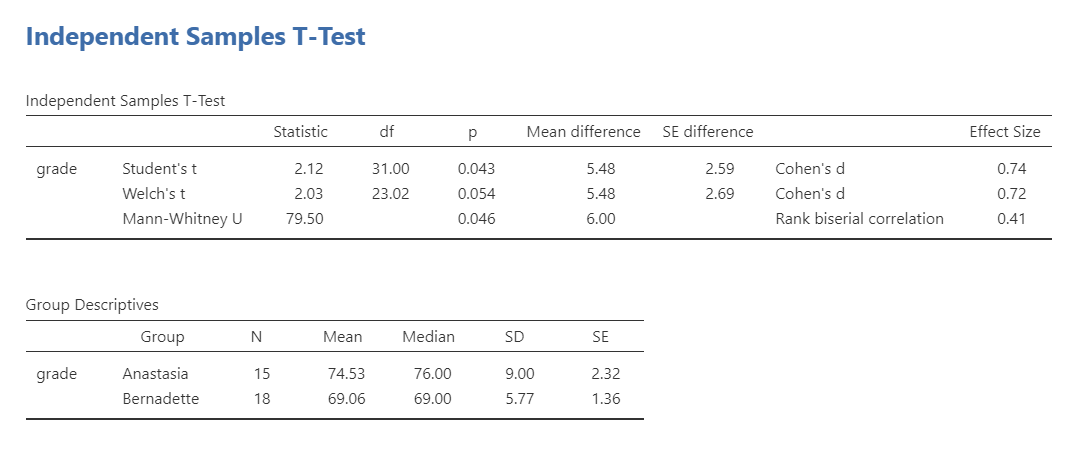
\includegraphics[width=1\linewidth]{images/02-independent_t-test/independent_t-test_full-results} 

}

\caption{All independent t-test results in jamovi}\label{fig:unnamed-chunk-5}
\end{figure}

\hypertarget{welchs-t-test-in-jamovi}{%
\subsubsection{Welch's t-test in jamovi}\label{welchs-t-test-in-jamovi}}

To conduct this in jamovi, under Tests select \texttt{Welch\textquotesingle{}s}. You will interpret the results similarly to the independent t-test:

\begin{quote}
Using a Welch's t-test, there was not a statistically significant difference in grades between Anastasia's students (\emph{M} = 74.53, \emph{SD} = 9.00, \emph{n} = 15) and Bernadette's students (\emph{M} = 69.06, \emph{SD} = 5.77, \emph{n} = 18), \emph{t} (23.02) = 2.03, \emph{p} = .054, \emph{d} = .72.
\end{quote}

Why is it no longer statistically significant? Which result should you trust? In reality, the difference in \emph{p}-values is likely due to chance. However, the independent t-test and Welch's test have different strengths and weaknesses. If the two populations really do have equal variances, then the independent t-test is slightly more powerful (lower Type II error rate) than the Welch's test. However, if they \emph{don't} have the same variances, then the assumptions of the independent t-test are violated and you may not be able to trust the results; you may end up with a higher Type I error rate. So it's a trade-off.

Which should you use? I tend to prefer always using Welch's t-test because if the variances are equal, then there will be practically no difference between the independent and Welch's t-test. But if the variances are not equal, then Welch's t-test will outperform the independent t-test. For that reason, defaulting to the Welch's t-test makes most sense to me.

\hypertarget{mann-whitney-u-test}{%
\subsubsection{Mann-Whitney U test}\label{mann-whitney-u-test}}

If you do not satisfy the assumption of normality (regardless of whether you satisfy the assumption of homogeneity of variance), you should either try to transform your data to be normally distributed or you will need to use a non-parametric test. In this case, if you originally wanted to perform an independent t-test, the non-parametric equivalent test is the Mann-Whitney U test.

I will not go into specifics, but the idea behind the Mann-Whitney U test is that you take all the values (regardless of group) and rank them. You then sum the ranks across groups and calculate your U statistic and p-value. You interpret the p-value like you normally would, but there are differences in how we report the results because this statistic is based on the \emph{median} not the \emph{mean}.

\begin{quote}
Using the Mann-Whitney U test, there was a statistically significant difference in grades between Anastasia's students (\emph{Mdn} = 76, \emph{n} = 15) and Bernadette's students (\emph{Mdn} = 69, \emph{n}~= 18), \emph{t} (23.02) = 2.03, \emph{p} = .054, \emph{d} = .72.
\end{quote}

\hypertarget{your-turn}{%
\section{Your turn!}\label{your-turn}}

Open the \texttt{Sample\_Dataset\_2014.xlsx} file that we will be using for all Your Turn exercises.

Perform independent t-tests based on the following research questions. Think critically about whether you should be using a one-tailed or two-tailed hypothesis and check your assumptions so you know which test to use!

To get the most out of these exercises, try to first find out the answer on your own and then use the drop-down menus to check your answer.

\begin{enumerate}
\def\labelenumi{\arabic{enumi}.}
\item
  \textbf{Does height differ by gender (Gender: male = 0, female = 1)?}

  \begin{itemize}
  \item
    Should you use a one-tailed or two-tailed hypothesis? one-tailed two-tailed
  \item
    Which statistic should you use based on your assumptions? independent t-test Welch's t-test Mann Whitney U
  \item
    Does height differ by gender? yes no
  \end{itemize}
\item
  \textbf{Do athletes (Athlete: athletes = 1, non-athlete = 0) have faster sprint times than non-athletes?}

  \begin{itemize}
  \item
    Should you use a one-tailed or two-tailed hypothesis? one-tailed two-tailed
  \item
    Which statistic should you use based on your assumptions? independent t-test Welch's t-test Mann Whitney U
  \item
    Do athletes have faster sprint times than non-athletes? yes no
  \end{itemize}
\item
  \textbf{Do students who live on campus (LiveOnCampus: on campus = 1, off campus = 0) have higher English scores than students who live off campus?}

  \begin{itemize}
  \item
    Should you use a one-tailed or two-tailed hypothesis? one-tailed two-tailed
  \item
    Which statistic should you use based on your assumptions? independent t-test Welch's t-test Mann Whitney U
  \item
    Does students who live on campus have higher English scores? yes no
  \end{itemize}
\item
  \textbf{Does athletic status relate to math scores?}

  \begin{itemize}
  \item
    Should you use a one-tailed or two-tailed hypothesis? one-tailed two-tailed
  \item
    Which statistic should you use based on your assumptions? independent t-test Welch's t-test Mann Whitney U
  \item
    Does athletic status relate to math scores? yes no
  \end{itemize}
\end{enumerate}

\hypertarget{dependent-t-test}{%
\chapter{Dependent t-test}\label{dependent-t-test}}

\hypertarget{what-is-the-dependent-t-test}{%
\section{What is the dependent t-test?}\label{what-is-the-dependent-t-test}}

The dependent t-test is used to test the difference in our dependent variable between two categories in which participants are the \emph{same} across categories. Our category variable is our independent variable. In other words, we use the independent t-test when we have a research question with a \textbf{continuous dependent variable} and a \textbf{categorical independent variable with two categories in which the same participants are in each category}.

The dependent t-test is also called a dependent samples t-test or paired samples t-test.

\hypertarget{data-set-up-1}{%
\section{Data set-up}\label{data-set-up-1}}

To conduct the dependent t-test, we first need to ensure our data is set-up properly in our dataset. This requires having two columns: one is our dependent variable score for the participant in one category and the other column is our dependent variable score for the participant in the other category. Each row is a unique participant or unit of analysis. Here's what example data may look like if we were testing for differences in test scores across the same participants in the fall and spring:

\begin{longtable}[]{@{}llr@{}}
\caption{Example data for the dependent t-test}\tabularnewline
\toprule
\begin{minipage}[b]{0.30\columnwidth}\raggedright
ID\strut
\end{minipage} & \begin{minipage}[b]{0.30\columnwidth}\raggedright
TestScore\_Fall\strut
\end{minipage} & \begin{minipage}[b]{0.30\columnwidth}\raggedleft
TestScore\_Spring\strut
\end{minipage}\tabularnewline
\midrule
\endfirsthead
\toprule
\begin{minipage}[b]{0.30\columnwidth}\raggedright
ID\strut
\end{minipage} & \begin{minipage}[b]{0.30\columnwidth}\raggedright
TestScore\_Fall\strut
\end{minipage} & \begin{minipage}[b]{0.30\columnwidth}\raggedleft
TestScore\_Spring\strut
\end{minipage}\tabularnewline
\midrule
\endhead
\begin{minipage}[t]{0.30\columnwidth}\raggedright
1\strut
\end{minipage} & \begin{minipage}[t]{0.30\columnwidth}\raggedright
75\strut
\end{minipage} & \begin{minipage}[t]{0.30\columnwidth}\raggedleft
86\strut
\end{minipage}\tabularnewline
\begin{minipage}[t]{0.30\columnwidth}\raggedright
2\strut
\end{minipage} & \begin{minipage}[t]{0.30\columnwidth}\raggedright
79\strut
\end{minipage} & \begin{minipage}[t]{0.30\columnwidth}\raggedleft
80\strut
\end{minipage}\tabularnewline
\begin{minipage}[t]{0.30\columnwidth}\raggedright
3\strut
\end{minipage} & \begin{minipage}[t]{0.30\columnwidth}\raggedright
65\strut
\end{minipage} & \begin{minipage}[t]{0.30\columnwidth}\raggedleft
75\strut
\end{minipage}\tabularnewline
\begin{minipage}[t]{0.30\columnwidth}\raggedright
4\strut
\end{minipage} & \begin{minipage}[t]{0.30\columnwidth}\raggedright
81\strut
\end{minipage} & \begin{minipage}[t]{0.30\columnwidth}\raggedleft
79\strut
\end{minipage}\tabularnewline
\begin{minipage}[t]{0.30\columnwidth}\raggedright
5\strut
\end{minipage} & \begin{minipage}[t]{0.30\columnwidth}\raggedright
73\strut
\end{minipage} & \begin{minipage}[t]{0.30\columnwidth}\raggedleft
82\strut
\end{minipage}\tabularnewline
\begin{minipage}[t]{0.30\columnwidth}\raggedright
6\strut
\end{minipage} & \begin{minipage}[t]{0.30\columnwidth}\raggedright
72\strut
\end{minipage} & \begin{minipage}[t]{0.30\columnwidth}\raggedleft
84\strut
\end{minipage}\tabularnewline
\begin{minipage}[t]{0.30\columnwidth}\raggedright
7\strut
\end{minipage} & \begin{minipage}[t]{0.30\columnwidth}\raggedright
69\strut
\end{minipage} & \begin{minipage}[t]{0.30\columnwidth}\raggedleft
90\strut
\end{minipage}\tabularnewline
\begin{minipage}[t]{0.30\columnwidth}\raggedright
8\strut
\end{minipage} & \begin{minipage}[t]{0.30\columnwidth}\raggedright
60\strut
\end{minipage} & \begin{minipage}[t]{0.30\columnwidth}\raggedleft
72\strut
\end{minipage}\tabularnewline
\begin{minipage}[t]{0.30\columnwidth}\raggedright
9\strut
\end{minipage} & \begin{minipage}[t]{0.30\columnwidth}\raggedright
75\strut
\end{minipage} & \begin{minipage}[t]{0.30\columnwidth}\raggedleft
75\strut
\end{minipage}\tabularnewline
\begin{minipage}[t]{0.30\columnwidth}\raggedright
10\strut
\end{minipage} & \begin{minipage}[t]{0.30\columnwidth}\raggedright
74\strut
\end{minipage} & \begin{minipage}[t]{0.30\columnwidth}\raggedleft
81\strut
\end{minipage}\tabularnewline
\bottomrule
\end{longtable}

In the example data above, what is your \textbf{independent variable}? ID Semester TestScore

In the example data above, what is your \textbf{dependent variable}? ID Semester Test Score

\hypertarget{the-math-behind-the-independent-t-test-1}{%
\section{The math behind the independent t-test}\label{the-math-behind-the-independent-t-test-1}}

The basic math of the dependent t-test is the mean difference divided by the standard error, which is estimated based on the standard deviation and sample size (N).

\(t = \frac{\bar{X}_1 - \bar{X}_2}{s_d/ \sqrt{N}}\)

\hypertarget{assumptions-1}{%
\section{Assumptions}\label{assumptions-1}}

As a parametric test, the independent t-test has the same assumptions as other parametric tests minus the homogeneity of variance assumption because we are dealing with the same people across categories

\begin{enumerate}
\def\labelenumi{\arabic{enumi}.}
\item
  The \emph{differences in scores} in the dependent variable are \textbf{normally distributed}
\item
  The dependent variable is \textbf{interval or ratio} (i.e., continuous)
\item
  Scores are \textbf{independent} across participants
\end{enumerate}

We cannot \underline{test} the second and third assumptions; rather, those are based on knowing your data.

However, we can and should test for the first assumption. Fortunately, the dependent samples t-test in jamovi has two check boxes under ``Assumption Checks'' that lets us test normality.

\hypertarget{in-jamovi-1}{%
\section{In jamovi}\label{in-jamovi-1}}

Let's run an example with data from lsj-data. Open data from your Data Library in ``lsj-data''. Select and open ``Chico''. This dataset is hypothetical data from Dr.~Chico's class in which students took two tests: one early in the semester and one later in the semester. Dr.~Chico thinks that the first test is a ``wake up call'' for students. When they realise how hard her class really is, they'll work harder for the second test and get a better mark. Is she right? Let's test it!

\begin{enumerate}
\def\labelenumi{\arabic{enumi}.}
\item
  To perform an dependent t-test in jamovi, go to the Analyses tab, click the T-Tests button, and choose ``Paired Samples T-Test''.
\item
  Move both measurements of your dependent variable (\texttt{grade\_test1} and \texttt{grade\_test2}) to the Paired Variables box.
\item
  Under Tests, select \texttt{Student\textquotesingle{}s}
\item
  Under Hypothesis, choose the correct hypothesis: Measure 1 is not equal to Measure 2 Measure 1 \textgreater{} Measure 2 Measure 1 \textless{} Measure 2
\item
  Under Additional Statistics, select \texttt{Mean\ difference}, \texttt{Effect\ size}, and \texttt{Descriptives}.
\item
  Under Assumption Checks, select both options: \texttt{Normality\ test} and \texttt{Q-Q\ plot}.
\end{enumerate}

When you are done, your setup should look like this

\begin{figure}

{\centering 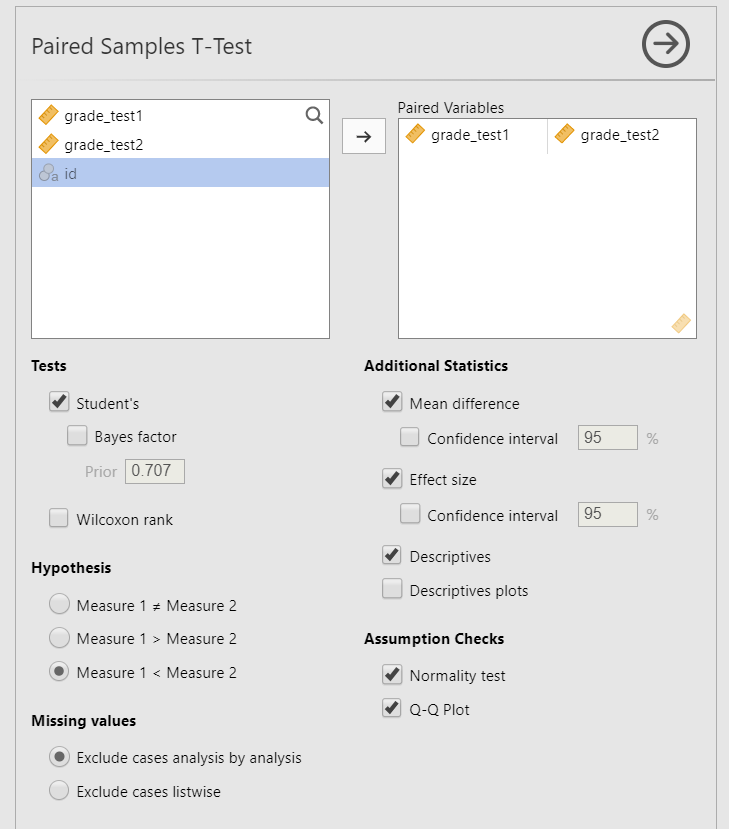
\includegraphics[width=0.8\linewidth]{images/03_dependent_t-test/dependent_setup} 

}

\caption{Dependent t-test setup in jamovi}\label{fig:unnamed-chunk-1}
\end{figure}

\hypertarget{checking-assumptions-in-jamovi-1}{%
\subsection{Checking assumptions in jamovi}\label{checking-assumptions-in-jamovi-1}}

\hypertarget{testing-normality-1}{%
\subsubsection{Testing normality}\label{testing-normality-1}}

We test for normality using the Shapiro-Wilk test and the Q-Q plot. The Shapiro-Wilk test was not statistically significant (W = .97, \emph{p} = .678); therefore, this indicates the data is normally distributed. Furthermore, the lines are fairly close to the diagonal line in the Q-Q plot (although it's a bit hard to tell because our sample size is small). We can conclude that we satisfy the assumption of normality.

\begin{figure}

{\centering 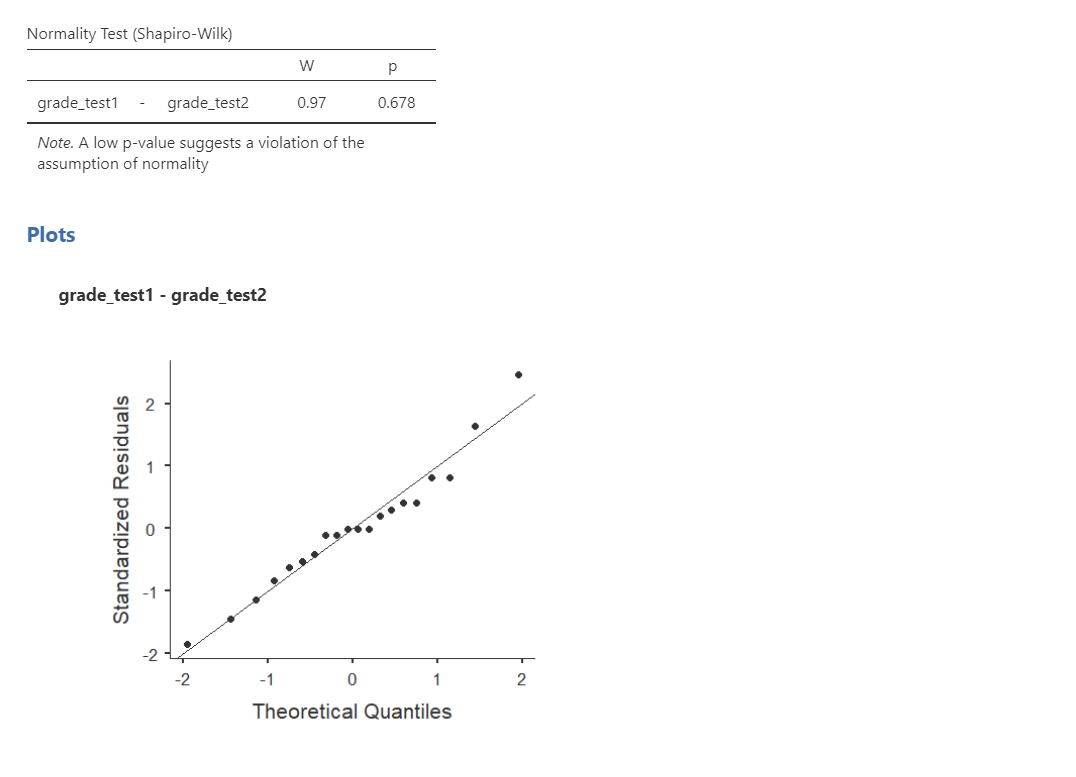
\includegraphics[width=1\linewidth]{images/03_dependent_t-test/dependent_normality} 

}

\caption{Testing normality in jamovi}\label{fig:unnamed-chunk-2}
\end{figure}

\hypertarget{interpreting-results-1}{%
\subsection{Interpreting results}\label{interpreting-results-1}}

Once we are satisfied we have satisfied the assumptions for the dependent t-test, we can interpret our results.

\begin{figure}

{\centering 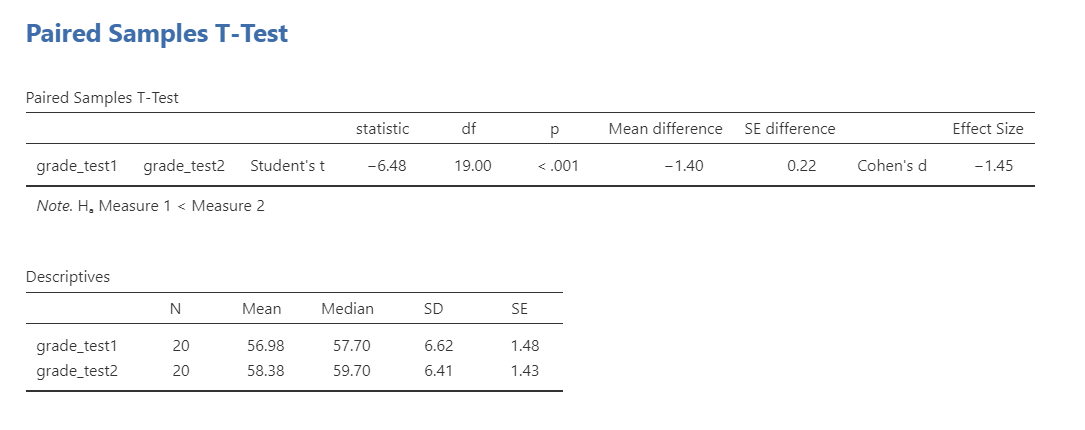
\includegraphics[width=1\linewidth]{images/03_dependent_t-test/dependent_results} 

}

\caption{Dependent t-test results in jamovi}\label{fig:unnamed-chunk-3}
\end{figure}

Our p-value is less than .05, so our results are statistically significant. We can write up our results in APA something like this:

\begin{quote}
The 20 students in Dr.~Chico's class performed worse on the first test (\emph{M} = 56.98, \emph{SD} = 6.62) than they did on the second test (\emph{M} = 58.38, \emph{SD} = 6.41), \emph{t}(19) = -6.48, \emph{p} \textless{} .001, \emph{d} = -1.45.
\end{quote}

Remember in the previous chapter that our t-test can be negative but we can always flip the interpretation. Here's another example of how we could write-up our results in APA style:

\begin{quote}
Dr.~Chico's hypothesis was correct in that her 20 students performed better on the second test (\emph{M} = 58.38, \emph{SD} = 6.41) than they did on the first test (\emph{M} = 56.98, \emph{SD} = 6.62), \emph{t}(19) = 6.48, \emph{p} \textless{} .001, \emph{d} = 1.45.
\end{quote}

\hypertarget{what-if-i-violated-assumptions-1}{%
\section{What if I violated assumptions?}\label{what-if-i-violated-assumptions-1}}

If you violated the assumption of normality and no transformation fixed your data, then you can perform the non-parametric version of the dependent t-test called the Wilcoxon Rank test. As a reminder, non-parametric tests do not make assumptions about the distribution of data because it deals with the \emph{median} not the \emph{mean}.

Here is the output for both the dependent t-test and the Wilcoxon rank test:

\begin{figure}

{\centering 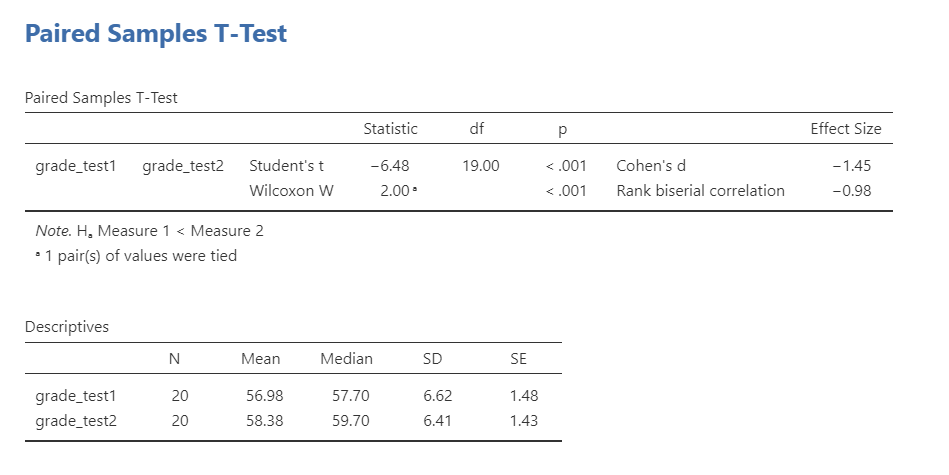
\includegraphics[width=1\linewidth]{images/03_dependent_t-test/dependent_results_full} 

}

\caption{All independent t-test results in jamovi}\label{fig:unnamed-chunk-4}
\end{figure}

\hypertarget{wilcoxon-rank-in-jamovi}{%
\subsubsection{Wilcoxon rank in jamovi}\label{wilcoxon-rank-in-jamovi}}

To conduct this in jamovi, under Tests select \texttt{Wilcoxon\ rank}. You will interpret the results similarly to the dependent t-test:

\begin{quote}
Using Wilcoxon rank test, students' test scores were significantly higher at the second test (\emph{Mdn} = 59.70) than at the first test (\emph{Mdn} = 57.70), W = 2.00, \emph{p} \textless{} .001.
\end{quote}

The note about tied values is not necessary to discuss. It is just telling us one participant had identical values for both test1 and test2 (student15).

\hypertarget{your-turn-1}{%
\section{Your turn!}\label{your-turn-1}}

Open the \texttt{Sample\_Dataset\_2014.xlsx} file that we use for all Your Turn exercises.

Perform dependent t-tests based on the following research questions. Think critically about whether you should be using a one-tailed or two-tailed hypothesis and check your assumptions so you know which test to use!

To get the most out of these exercises, try to first find out the answer on your own and then use the drop-down menus to check your answer.

\textbf{Note}: Technically, none of our data is suitable for a dependent t-test in this dataset. We will pretend that the four test score variables (\texttt{English}, \texttt{Reading}, \texttt{Math}, and \texttt{Writing}) are really four measurements of the same underlying test. In reality, we would analyze this data using correlation.

\begin{enumerate}
\def\labelenumi{\arabic{enumi}.}
\item
  \textbf{Do students perform better on the English test than they do the Writing test?}

  \begin{itemize}
  \item
    Should you use a one-tailed or two-tailed hypothesis? one-tailed two-tailed
  \item
    Which statistic should you use based on your assumptions? dependent t-test Wilcoxon rank
  \item
    Do students perform better on the English test than they do the Writing test? yes no
  \end{itemize}
\item
  \textbf{Does students' English scores relate to their Reading scores?}

  \begin{itemize}
  \item
    Should you use a one-tailed or two-tailed hypothesis? one-tailed two-tailed
  \item
    Which statistic should you use based on your assumptions? dependent t-test Wilcoxon rank
  \item
    Does students' English scores relate to their Reading scores? yes no
  \end{itemize}
\end{enumerate}

\hypertarget{appendix-appendices}{%
\appendix}


\hypertarget{references}{%
\chapter{References}\label{references}}

  \bibliography{book.bib,packages.bib}

\end{document}
